%!TEX root = thesis.tex
\chapter{Introduction}\label{chap:intro} 

\section{Background of the Study}

Market behavior is shaped not only by price movements but also by the broader economic context that affects risk, liquidity, and investor behavior. Over the past decade, computer vision-based models have become a popular tool that convert price data into images and train Convolutional Neural Networks (CNN) to generate \textit{Buy/Hold/Sell} decisions \cite{cohen2020trading,sezer2018algorithmic,gudelek2017deep}. These are effective in capturing local patterns of time and price. However they usually treat the macroeconomic context separately, which has a clear contribution to changing market prices \cite{wang2019aggregating,ma2022macroeconomic,chauhan2025exploring}.

This study aims to improve existing image-based representations by merging technical and macroeconomic indicators into a unified image representation so that it can be processed by our proposed CNN model. 
The model takes into account strict time adaptation, uniform normalization, and careful encoding to preserve the relationship between local patterns and market context \cite{sezer2018algorithmic,maratkhan2021deep}. 
The framework is applied to selected Philippine blue-chip, penny stocks, and cryptocurrency, where the impact of incorporating macroeconomic indicators on prediction accuracy and performance metrics is measured.


\section{Basic Definitions and Notations}\label{sec:BasicDefns}
\subsubsection*{Quantitative Trading using Image Classification}
Quantitative trading is a system that automates trades that are conducted using models and technical indicators as tools \cite{ta2018prediction}. It can be represented in images that are in a grid of indicators and time windows, to allow spatial filters to uncover patterns that match price movement \cite{cohen2020trading,sezer2018algorithmic}. Representations such as candlesticks, bar charts, and technical indicators as images can improve trend classification and transaction signals \cite{gudelek2017deep,chen2020encoding,liu2023automated}. Transforming financial time series into visual representations enables machine learning algorithms to efficiently recover complex trading signals \cite{cohen2020trading}, with candlestick image data consistently outperforming traditional numeric approaches \cite{liu2023automated}. 


\subsubsection*{CNN-based Technical Indicator Clustering (CNN--TIC)}

Convolutional neural networks are structured to learn spatial patterns from grid-formatted data, which makes them well suited for technical indicators arranged as two-dimensional images \cite{al2017understanding,lecun1995learning}. Early image-based trading studies demonstrated that converting technical indicators into fixed-size grayscale images allows a CNN to detect local price and momentum patterns more effectively than traditional numeric inputs \cite{sezer2018algorithmic}. This established image representation as a practical way to capture short-term market patterns.

Later work organized technical indicators into clustered channels, forming what is now known as the CNN--TIC model \cite{maratkhan2021deep}. In that model, fifteen technical indicators were used to represent market behavior: Relative Strength Index (RSI), Williams~\%R, Simple Moving Average (SMA), Exponential Moving Average (EMA), Weighted Moving Average (WMA), Hull Moving Average (HMA), Triple Exponential Moving Average (TEMA), Commodity Channel Index (CCI), Chande Momentum Oscillator (CMO), Moving Average Convergence Divergence (MACD), Percentage Price Oscillator (PPO), Rate of Change (ROC), Chaikin Money Flow Indicator (CMFI), Directional Movement Indicator (DMI), and Parabolic Stop and Reverse Indicator (PSI) \cite{maratkhan2021deep}.

These indicators describe different aspects of price behavior. RSI, Williams~\%R, CCI, CMO, MACD, PPO, ROC, DMI, and PSI measure momentum, trend direction, or possible reversal behavior. SMA, EMA, WMA, HMA, and TEMA describe smoothed price trends using different weighting schemes. CMFI adds volume information by estimating whether buying or selling pressure is supported by trading volume. In general, these indicators are derived from OHLCV data through moving averages, price differences, high--low ranges, momentum ratios, or volume-weighted price relationships over a defined lookback window \cite{wilder1978new,murphy1999technical,achelis2001technical}.

In CNN--TIC, these indicators were grouped into separate channels based on similarity in behavior, allowing the model to process related technical indicators within the same representation \cite{maratkhan2021deep}. This makes CNN--TIC an appropriate baseline for this study, since it uses image-based technical indicator representations for Buy, Hold, and Sell classification.

\subsubsection*{Multimodal Approach}
In deep learning, multimodal processing refers to the integration of data from different types to increase the learning efficiency and performance of algorithms on a specific task \cite{dimitri2022short}. This approach is advantageous because each modality responds to different characteristics and provides complementary information that is not fully captured by a single form of data. For example, visual data can support and validate the content of spoken language, while textual data can explain the content of visual cues. In the context of the financial market, the technical picture from OHLCV (Open, High, Low, Close, Volume) data depicts local patterns over time and price, while textual policy statements, earnings reports, and sentiment measures on social media provide a more slowly evolving context of market environment and risk \cite{farimani2024adaptive,karadacs2025multimodal}.

These representations provide a broader range of signals that can help to understand the change and risk of the market environment \cite{zhang2020multimodal}. Fusion can be viewed as the combination of different modalities into a single meaning space, so that the learned patterns are richer, more robust to noise, and more appropriate to different market conditions. Additionally, it can also be presented in a form that is well-suited for learning that can improve classification and prediction compared to relying on a single approach \cite{gallo2018image}. 

\subsubsection*{Macroeconomic Representation}
Macroeconomic representations are economic signals such as interest rates, inflation, exchange rates, market volatility, and foreign investment, that reflect the state of the market environment at a given time \cite{artantacs2020selected}. These indicators represent the broader economic conditions that influence market behavior, investor sentiments, liquidity, and overall financial returns \cite{Naik02012024,mazumder2025impact}. This is relevant because literature shows that macroeconomic attention and policy uncertainty are significantly linked to expected short- and long-term earnings and sector dynamics \cite{ma2022macroeconomic}. In this view, the macro series becomes the “context” that moves slowly and shapes the course of the market and liquidity, while technical indicators from OHLCV represent the faster, more localized patterns. It is important to describe these signals in a consistent form and scale that can be related to the technical representation \cite{wang2019aggregating}.

For this study, five macroeconomic indicators were selected: Reverse Repurchase Rate (RRP), gold price, crude oil price, purchasing power of the peso (PPP), and inflation rate. The RRP represents the monetary policy stance of the Bangko Sentral ng Pilipinas and reflects the rate used in its reverse repurchase operations \cite{bsp2025rrp}. Gold price was included as an indicator of uncertainty and store-of-value demand, while crude oil price was included because energy prices affect production costs, inflation pressure, and broader economic activity \cite{worldbank2025commoditymarkets,mazumder2025impact}. PPP refers to the purchasing power of the peso which represents the real value of the peso relative to a reference period using the Consumer Price Index \cite{psa2020ppp}. Inflation rate was included because it measures changes in consumer prices and reflects the price stability of the economy \cite{psa2025cpi}.

Together, these indicators provide a compact representation of the macroeconomic setting surrounding each trading day. RRP captures monetary policy conditions, gold captures uncertainty-related conditions, crude oil captures energy-related cost pressure, PPP captures the real value of the peso, and inflation captures general price movement. These variables are aligned with the trading calendar and normalized into a common grayscale range so that CNN--MIC can process macroeconomic context together with technical patterns in a single image representation.

\section{Problem Statement}\label{sec:ResearchQ}
\begin{figure}[H]
	\centering
	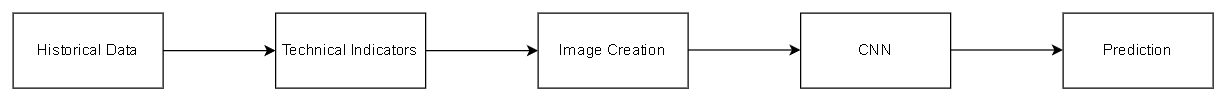
\includegraphics[width=0.8\textwidth]{../figures/CNN-TIC.png}
	\caption{Computer-vision trading using technical indicators}
	\label{Figure 1: Computer-vision trading using technical indicators}
\end{figure}


Figure~\ref{Figure 1: Computer-vision trading using technical indicators}  illustrates a typical single-mode workflow where historical price data are transformed into technical indicators, arranged as two-dimensional images, and passed through a CNN to generate trading signals \cite{sezer2018algorithmic,gudelek2017deep}. This setup is effective in capturing local price-time patterns because convolutional filters can highlight short-term structures on the image \cite{cohen2020trading}. However, the representation is restricted to indicators derived from OHLCV and does not explicitly incorporate macroeconomic information that shapes market risk, liquidity, and trend formation.

As a result, current CNN-based image models provide an incomplete view of the market environment. Broader conditions such as changes in interest rates, inflation, or policy-related uncertainty are not encoded in the same space as the technical picture, even if they have a documented effect on asset returns \cite{wang2019aggregating,ma2022macroeconomic,chauhan2025exploring}. In simple terms, existing CNN trading systems operate only on technical indicator images, and there is no unified image representation where technical signals and macroeconomic indicators are jointly organized, aligned, and scaled. This gap is the main problem that the study aims to address.

\section{Aim of the Work}
\subsection{General Objective}

\noindent Develop and evaluate an enhanced CNN-based trading model that integrates both technical and macroeconomic indicators to assess their effect on financial market trend prediction and trading performance.

\subsection{Specific Objectives}
\begin{enumerate}
	\item To enhance the CNN--TIC framework by expanding its technical indicator image matrix to include macroeconomic variables, forming a unified visual representation.
	\item To compare model performance using metrics such as accuracy, F1-score, and annualized return, to determine whether the inclusion of macroeconomic indicators leads to significant improvements.
	\item To evaluate performance on different stock categories in the PSE market and cryptocurrency.
	\item To evaluate feature importance and model behavior, interpret how macroeconomic information contributes to CNN decision-making in the context of financial trend prediction.
\end{enumerate}


\subsection{Scope and Limitation}
Previous studies on quantitative trading involve only CNNs that are solely trained on technical indicators as image representations. In such settings, the absence of macroeconomic information may limit the robustness and accuracy of the resulting models. Thus, this study aims to develop and evaluate a CNN-based trading framework that integrates both technical and macroeconomic indicators into a single image representation for market trend prediction.

The model will be tested on different stocks of the Philippine Stock Exchange (PSE) market, and will further include cryptocurrency data. The dataset will include historical daily price data, trading volumes, and selected macroeconomic indicators such as reverse repurchase (RRP), purchasing power of peso, inflation rate, gold, and crude oil. Meanwhile, the technical indicators that will be used are  Relative Strength Index (RSI), Williams~\%R, Simple Moving Average (SMA), Exponential Moving Average (EMA), Weighted Moving Average (WMA), Hull Moving Average (HMA), Triple Exponential Moving Average (TEMA), Commodity Channel Index (CCI), Chande Momentum Oscillator (CMO), Moving Average Convergence Divergence (MACD), Percentage Price Oscillator (PPO), Rate of Change (ROC), Chaikin Money Flow Indicator (CMFI), Directional Movement Indicator (DMI), and Parabolic Stop and Reverse Indicator (PSI).

Although quantitative trading is focused on financial market prediction, this study will only focus on stock data from the Philippine market, which may limit its applicability to other stock markets with different economic conditions. Additionally, trading simulations used a fixed commision of 50 pesos per trade and ignores market slippage. Nonetheless, this study aims to develop a structured framework to identify how macroeconomic integrated visual representations can enhance CNN-based trading performance across various market conditions.

\subsection{Significance of the Study}
With the growing interest in applying computer vision for market trend prediction, the need to show how we can incorporate both technical and macroeconomic indicators into a single image representation becomes even more important. Unlike traditional CNN models that solely rely on technical indicators, the proposed CNN framework aims to improve predictive accuracy and financial returns across different market conditions that are driven by macroeconomic factors.

The research will contribute to developing more adaptive quantitative trading systems that supports data-driven decision-making for traders and financial institutions. Academically, it extends computer vision applications in finance and provides a reproducible foundation for future studies on financial forecasting.




